\section{Methods}\label{sec:methods}

The study was built in ten steps (Table~\ref{tab:steps}). We describe them in the order in which they were carried out, because several design decisions only make sense as responses to what an earlier step revealed. Section~\ref{sec:results} reports the output of each step under the same numbering.

\begin{table}[ht]
\centering\small
\caption{The ten steps of the study, and where each is described and reported.}\label{tab:steps}
\begin{tabularx}{\textwidth}{@{}c>{\raggedright\arraybackslash}p{5.2cm}>{\raggedright\arraybackslash}X@{}}
\toprule
Step & What was done & Real output shown \\
\midrule
0 & Data selection and sampling & Sample composition (Table~\ref{tab:sample}) \\
1 & Feasibility spike with a stand-in renderer & Recovered fraction of record, beats found \\
2 & Official rendering tool on a real record & Rendered page; layout-match score; heart rate \\
3 & Six-record validation & Table~\ref{tab:step3}, Fig.~\ref{fig:step3} \\
4 & Degradation model & Fig.~\ref{fig:grid}, Table~\ref{tab:degradation} \\
5 & Harness and pilot (10 records, blur) & Throughput; error vs blur; one bug \\
6 & Sweep 1: 1{,}550 tests, checkpointed & Cleaning table; reliability (Fig.~\ref{fig:fig3}) \\
7 & Sweep 1 analysis: heart rate and outcomes & Figs.~\ref{fig:fig1}--\ref{fig:fig2} \\
8 & Sweep 2: PR, QRS, QT, QTc & Completion; data dictionary \\
9 & Sweep 2 analysis and cross-checks & Figs.~\ref{fig:ba}--\ref{fig:intervals}, Tables~\ref{tab:intervals}--\ref{tab:tests} \\
\bottomrule
\end{tabularx}
\end{table}

\subsection{Step 0: data and sampling}
\textbf{Data.} We used PTB-XL v1.0.3 \citep{ref45}, a public 12-lead ECG dataset of 21{,}799 ten-second records from 18{,}869 patients, released under CC-BY 4.0 with diagnostic annotations. The low-resolution (100\,Hz) files were used for rendering and for the sweeps; the 500\,Hz files were used only for the ground-truth sampling-rate check in Section~\ref{sec:gt500}.

\textbf{Labels.} Each record's diagnostic superclass was taken from its highest-likelihood SCP code, mapped through the dataset's statement table. A record was labelled \emph{abnormal} if it had a superclass other than NORM, and \emph{normal} otherwise. One sampled record has a dominant code with no diagnostic superclass and is therefore counted as normal by this rule (Table~\ref{tab:sample}).

\textbf{Sampling.} Because false reassurance can only be observed on a record whose truth is abnormal, sampling was stratified. A pool of 500 records (250 normal, 250 abnormal) was drawn with a fixed random seed (42) and saved; the study sample is a fixed 50-record subset of that pool (25 normal, 25 abnormal, seed 42). \textbf{The sample size was reduced from a planned $\approx$500 records to 150 and then to 50} because 500 records $\times$ 31 versions was estimated at $\approx$87 GPU-hours, which did not fit the free GPU quota or the project deadline; 50 records was estimated at $\approx$10.5 hours. This reduction was decided before any result was seen. The pool, seed and selection code are fixed so the sample can be regenerated exactly (the analysis script reconstructs it from the public metadata).

\begin{table}[ht]
\centering\small
\caption{Composition of the 50-record sample. Sex and age from PTB-XL metadata.}\label{tab:sample}
\begin{tabular}{@{}lr@{\qquad}lr@{}}
\toprule
Diagnostic superclass & Records & Attribute & Value \\
\midrule
NORM & 24 & Male / female & 24 / 26 \\
HYP (hypertrophy) & 9 & Median age (years) & 63 \\
STTC (ST/T change) & 7 & Age range (years) & 26 to $>$89$^{\dagger}$ \\
CD (conduction disturbance) & 5 & Labelled normal / abnormal & 25 / 25 \\
MI (myocardial infarction) & 4 & & \\
No superclass & 1 & & \\
\bottomrule
\end{tabular}

\smallskip
\footnotesize $^{\dagger}$PTB-XL stores ages above 89 as 300 to protect identity; one sampled patient carries that code, and it is not an age.
\end{table}

\subsection{Software environment and its limits}
Development was done on a Windows~11 laptop without a GPU, using Python~3.14 in an isolated virtual environment for the core scientific stack (NumPy, SciPy, pandas, Matplotlib, OpenCV, \texttt{wfdb}, NeuroKit2, PyTorch~2.13). ECG-Image-Kit requires older libraries that do not exist for Python~3.14, so it was run in a second, separate Python~3.11 environment. The two sweeps ran in Google Colab on a T4 GPU (Python~3.13). Analysis scripts were run locally with SciPy~1.18.1.

\textbf{What was not recorded.} The exact commit hashes of ECG-Image-Kit and Open-ECG-Digitizer, and the exact library versions inside each Colab session, were not recorded. The digitiser was cloned from its public repository at the start of every session without pinning a version. Section~\ref{sec:drift} shows that this mattered. We report it here so that a reader does not assume a pinned environment.

\subsection{Step 1: feasibility spike (one record, stand-in renderer)}
Before committing to the toolchain, one record (PTB-XL \texttt{00001\_lr}, 12 leads, 10\,s) was pushed through the whole chain with throw-away code: render an ECG page, digitise it, compute a heart rate, compare with the record's own value. The official renderer could not be installed on the main Python (see Step~2), so a small stand-in script drew the signal on a printed-paper-style grid. The digitiser also refused to start because its top-level imports pulled in a training-only library (Ray) that does not exist for Python~3.14. Inspection of its source confirmed that only a training helper used it, so the import was made optional in the local copy (one commented edit, no change to inference code).

\subsection{Step 2: official rendering tool}
ECG-Image-Kit \citep{ref1} was installed in the Python~3.11 environment. Its optional handwriting-annotation feature depends on a TensorFlow build that is unavailable and on a compiler that was not installed; because that feature is not used here, the import was made conditional on the feature being requested. The interim run had appeared to succeed, but reading the full installation log showed that a required package had silently failed to install; a shortened view of the log (its last lines) had hidden this. All later installs were checked against the complete log. The tool then rendered the same record as a correctly formatted 12-lead page with grid, lead labels, calibration pulses and a rhythm strip.

\subsection{Step 3: six-record validation}
Six records (\texttt{00001}--\texttt{00006}) were rendered and digitised. For each, lead~II heart rate was computed from the ground-truth signal and from the digitised signal (Section~\ref{sec:metrics}) and compared. These six records were chosen for convenience (the first six in the dataset), are undamaged, and are not part of the 50-record sample.

\subsection{Step 4: degradation model}\label{sec:degradation}
Each clean rendered page was degraded with OpenCV along six axes chosen to span distinct photographic failure modes: focus, camera angle, storage or transmission, camera distance, ambient light, and print condition (Table~\ref{tab:degradation}, Fig.~\ref{fig:grid}). Each axis has five levels of increasing severity plus the shared clean image, giving $6\times5+1=31$ versions per record. One axis is varied at a time; combinations were not tested. Degradation is applied to the whole page, as it would be to a photograph, and the digitiser receives the whole page.

\begin{table}[ht]
\centering\small
\caption{Degradation axes, what each simulates, and the parameter at each level (OpenCV implementation).}\label{tab:degradation}
\begin{tabularx}{\textwidth}{@{}lXl@{}}
\toprule
Axis & Implementation & Levels 1--5 \\
\midrule
Blur & Gaussian blur, square kernel (px) & 3, 7, 11, 15, 21 \\
Tilt & Rotation about page centre, white fill (degrees) & 2, 5, 8, 12, 16 \\
JPEG & Re-encode at JPEG quality & 50, 30, 15, 8, 3 \\
Resolution & Downscale by factor (area), then upscale back (linear) & $\times$0.75, 0.5, 0.35, 0.25, 0.15 \\
Uneven lighting & Horizontal linear brightness gradient, darkest fraction at the right edge & 15, 30, 45, 60, 75\,\% \\
Grid contrast & Blend each pixel toward the image mean by fraction $s$ & 15, 30, 45, 60, 75\,\% \\
\bottomrule
\end{tabularx}
\end{table}

\begin{figure}[ht]
\centering
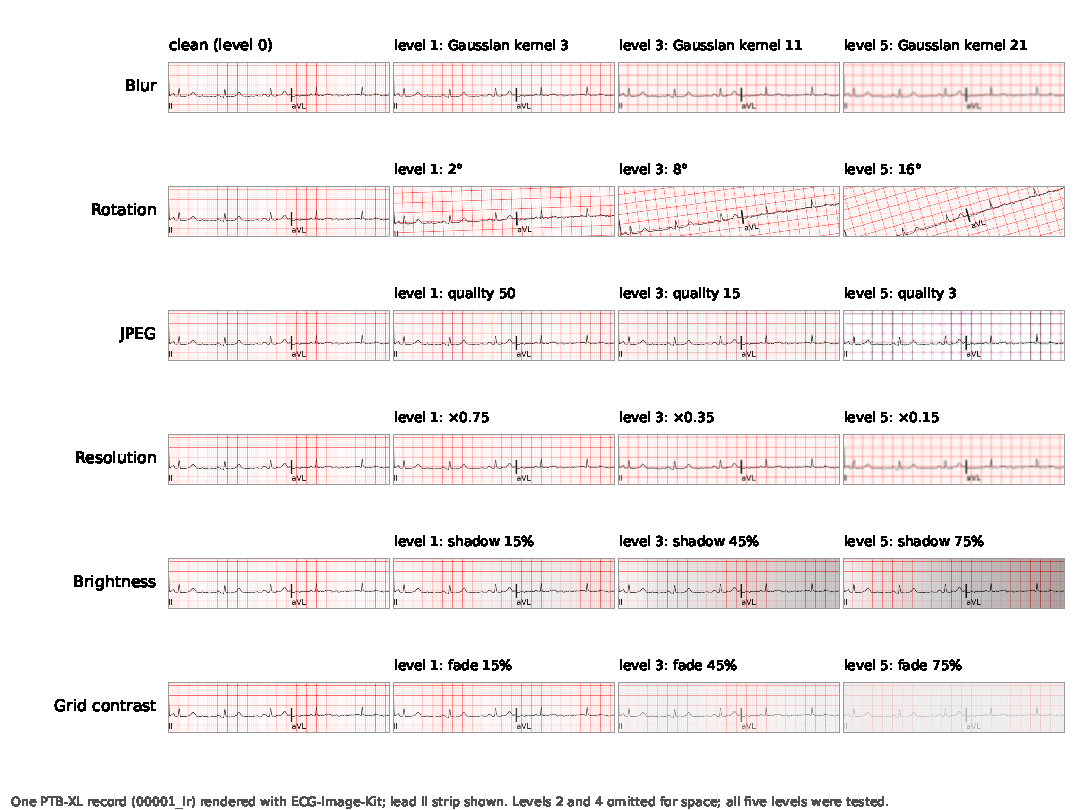
\includegraphics[width=\textwidth]{figures/fig_degradation_grid.pdf}
\caption{One real record (PTB-XL \texttt{00001\_lr}) rendered with ECG-Image-Kit and degraded exactly as in the sweep (the code that produced this figure reuses the sweep's functions). Levels 0, 1, 3 and 5 of every axis are shown, cropped to the lead~II strip; for tilt the crop follows the trace. Levels 2 and 4 were also tested.}\label{fig:grid}
\end{figure}

\subsection{Step 5: harness and pilot}
The chain was rebuilt as a notebook for Google Colab, because the local environment had by then been found to be broken (its configuration pointed at another machine's user profile). The pilot ran 10 records $\times$ blur $\times$ 6 levels (clean plus five) $=60$ tests. It served two purposes: to prove that sampling, rendering, degradation, digitisation and comparison work end to end, and to measure throughput before committing to the full sweep.

\subsection{Step 6: sweep 1 (heart rate)}\label{sec:sweep1}
Sweep~1 processed the 50-record sample $\times$ 31 versions $=1{,}550$ tests, digitising each page with Open-ECG-Digitizer and computing lead~II heart rate against ground truth. Everything that had to survive a session disconnect (the record sample, the rendered clean pages, and the results table) was stored on Google Drive. Tests were processed in sub-batches of 20; after every sub-batch the results file was written to a temporary file, swapped in atomically, copied to a time-stamped backup, and \emph{read back from Drive} with an assertion that the row count matched memory. This verified-save design was adopted after a stale browser view made a complete results file look as if $\approx$500 tests had been lost. The notebook prints the compute device at start, because newly uploaded notebooks default to CPU and this was missed three times.

\subsection{Step 7: Sweep 1 analysis}\label{sec:sweep1analysis}
Sweep~1 was analysed in Colab notebooks that read the checkpointed results file. They (i) removed duplicate and stray rows and counted unreadable tests (cleaning), (ii) identified the records that failed to digitise, separating failures on the clean image from failures caused by damage, (iii) classified each heart rate as slow ($<60$\,bpm), normal (60--100\,bpm) or fast ($>100$\,bpm) and tabulated the outcomes described in Section~\ref{sec:metrics}, and (iv) drew the figures. Records that failed to digitise were reported separately and excluded from the damage curves, leaving the reliable set.

\subsection{Step 8: sweep 2 (heart rate and intervals)}\label{sec:sweep2}
Sweep~1 discarded each digitised waveform after computing heart rate, so PR, QRS, QT and QTc could not be recovered from it. Sweep~2 therefore re-digitised every image from scratch, over the \emph{same} 50 records (same pool, same seed), and additionally extracted PR, QRS, QT and QTc from both signals (Section~\ref{sec:metrics}) and looked up patient sex for the sex-specific QTc threshold. It wrote to a separate results file so that Sweep~1's verified results could not be affected. The interval-extraction function was unit-tested on a synthetic ECG, and the full metric function was dry-run against mock ground-truth and digitised data extracted verbatim from the built notebook, before any GPU time was used.

\subsection{Step 9: Sweep 2 analysis and cross-checks}\label{sec:sweep2analysis}
Sweep~2 was analysed locally with Python scripts (Appendix~\ref{sec:repro}). They repeated the Sweep~1 analysis on the new file, added the interval error tables and the QTc outcome, and ran the cross-checks that the earlier steps had made necessary: the paired tests and Bland--Altman analysis (Section~\ref{sec:stats}), the recomputation of ground truth at 500\,Hz, the breakdown by diagnostic superclass, and a test-by-test comparison of the two sweeps.

\subsection{Metrics}\label{sec:metrics}
\textbf{Ground truth and digitised signals.} Ground truth is lead~II of the PTB-XL 100\,Hz record. The digitiser returns a 1{,}000\,Hz time series per lead in microvolts (converted to millivolts). Only lead~II was analysed. If the digitiser returned no signal, the test is a \emph{silent drop}.

\textbf{Heart rate.} R peaks were detected with NeuroKit2 and heart rate taken as the mean instantaneous rate over the record. Heart-rate error is the absolute difference between digitised and ground-truth values.

\textbf{Intervals.} After NeuroKit2 signal cleaning, R peaks were detected and P, QRS and T boundaries located with the discrete-wavelet delineator. At least three R peaks were required. PR is the mean over beats of (R-onset $-$ P-onset), QRS duration the mean of (R-offset $-$ R-onset), and QT the mean of (T-offset $-$ R-onset). QTc uses Bazett's correction with the test's own detected heart rate. As a sensitivity check on the QTc outcome analysis, Fridericia's correction (QT$/$RR$^{1/3}$) was also applied: the truly prolonged records fell from 21 to 16 and the real false-reassurance events from 6 to 2 (overlapping Wilson 95\% intervals; unchanged with a 20\,ms instead of 10\,ms tolerance), so the Bazett count is best read as an upper bound. Interval error is the absolute difference between digitised and ground-truth values. Ground-truth intervals were computed from the 100\,Hz records in the sweep and recomputed from the 500\,Hz records for the analysis in Section~\ref{sec:gt500}; intervals in the main results use the 500\,Hz version.

\textbf{Patient-facing outcome (heart rate).} A heart rate is banded as slow ($<$60\bpm), normal (60--100\bpm) or fast ($>$100\bpm) \citep{ref52}. Comparing the digitised band with the ground-truth band gives: correct; false alarm (normal truth, abnormal reading); \textbf{false reassurance} (abnormal truth, normal reading); wrong-abnormal; or silent drop. A false reassurance is counted as \emph{real} only if the digitised value is more than 10\bpm\ from the truth. A smaller discrepancy that crosses the band edge (for example 59.7 read as 60.0\bpm) is a \emph{boundary flip}, reported separately.

\textbf{Patient-facing outcome (QTc).} QTc was classed prolonged if it exceeded 460\,ms in women or 450\,ms in men \citep{ref52}, using PTB-XL sex. The same outcome categories apply, with two additions found necessary during analysis (Section~\ref{sec:qtcoutcome}): an event counts as real only if (a) it exceeds 10\,ms and (b) the same record's own \emph{clean} image was classified correctly, because a record already misclassified without any degradation cannot demonstrate a degradation effect.

\textbf{Reliable records.} A record was \emph{reliable} if the digitiser returned a heart rate for at least 25 of its 31 versions ($\le$6 unreadable, $\le$20\,\%). Degradation analyses use reliable records only; excluded records are reported separately.

\textbf{Signal-to-noise ratio.} The sweep code also computed a signal-to-noise value. We do \emph{not} report it. The computation compared the 100\,Hz ground truth and the 1{,}000\,Hz digitised signal sample by sample without resampling or time alignment, and its median on undamaged images was about $-3$\,dB, which is not meaningful. This was discovered only when preparing this paper.

\subsection{Statistical analysis}\label{sec:stats}
Errors are skewed, so we report medians with interquartile ranges (IQR) and, where a mean is informative, means. Each degraded level was compared with the \emph{same record's} clean image using a paired Wilcoxon signed-rank test, with Holm correction across the $6\times5=30$ comparisons of each metric; the effect size is the median paired excess error. Because statistical significance with 49 records can be reached for negligible effects, we always report the effect size beside it. Confidence intervals for proportions are Wilson intervals. Agreement between digitised and ground-truth values on clean images is summarised with Bland--Altman bias and 95\,\% limits of agreement. Sex-, age- and class-adjusted models were not fitted, because the number of records is too small to support them.
